\documentclass[12pt,a4paper]{report}
\usepackage{graphicx}
\usepackage{pdfpages}
\usepackage{hyperref}
\usepackage{wrapfig}
\usepackage{lscape}
\usepackage{rotating}
\usepackage{epstopdf}
\usepackage[utf8]{inputenc}
\usepackage[cyr]{aeguill}
\usepackage[francais]{babel}
\graphicspath{ {images/} }
\hypersetup{
    colorlinks,
    citecolor=black,
    filecolor=black,
    linkcolor=black,
    urlcolor=black
}
\begin{document}
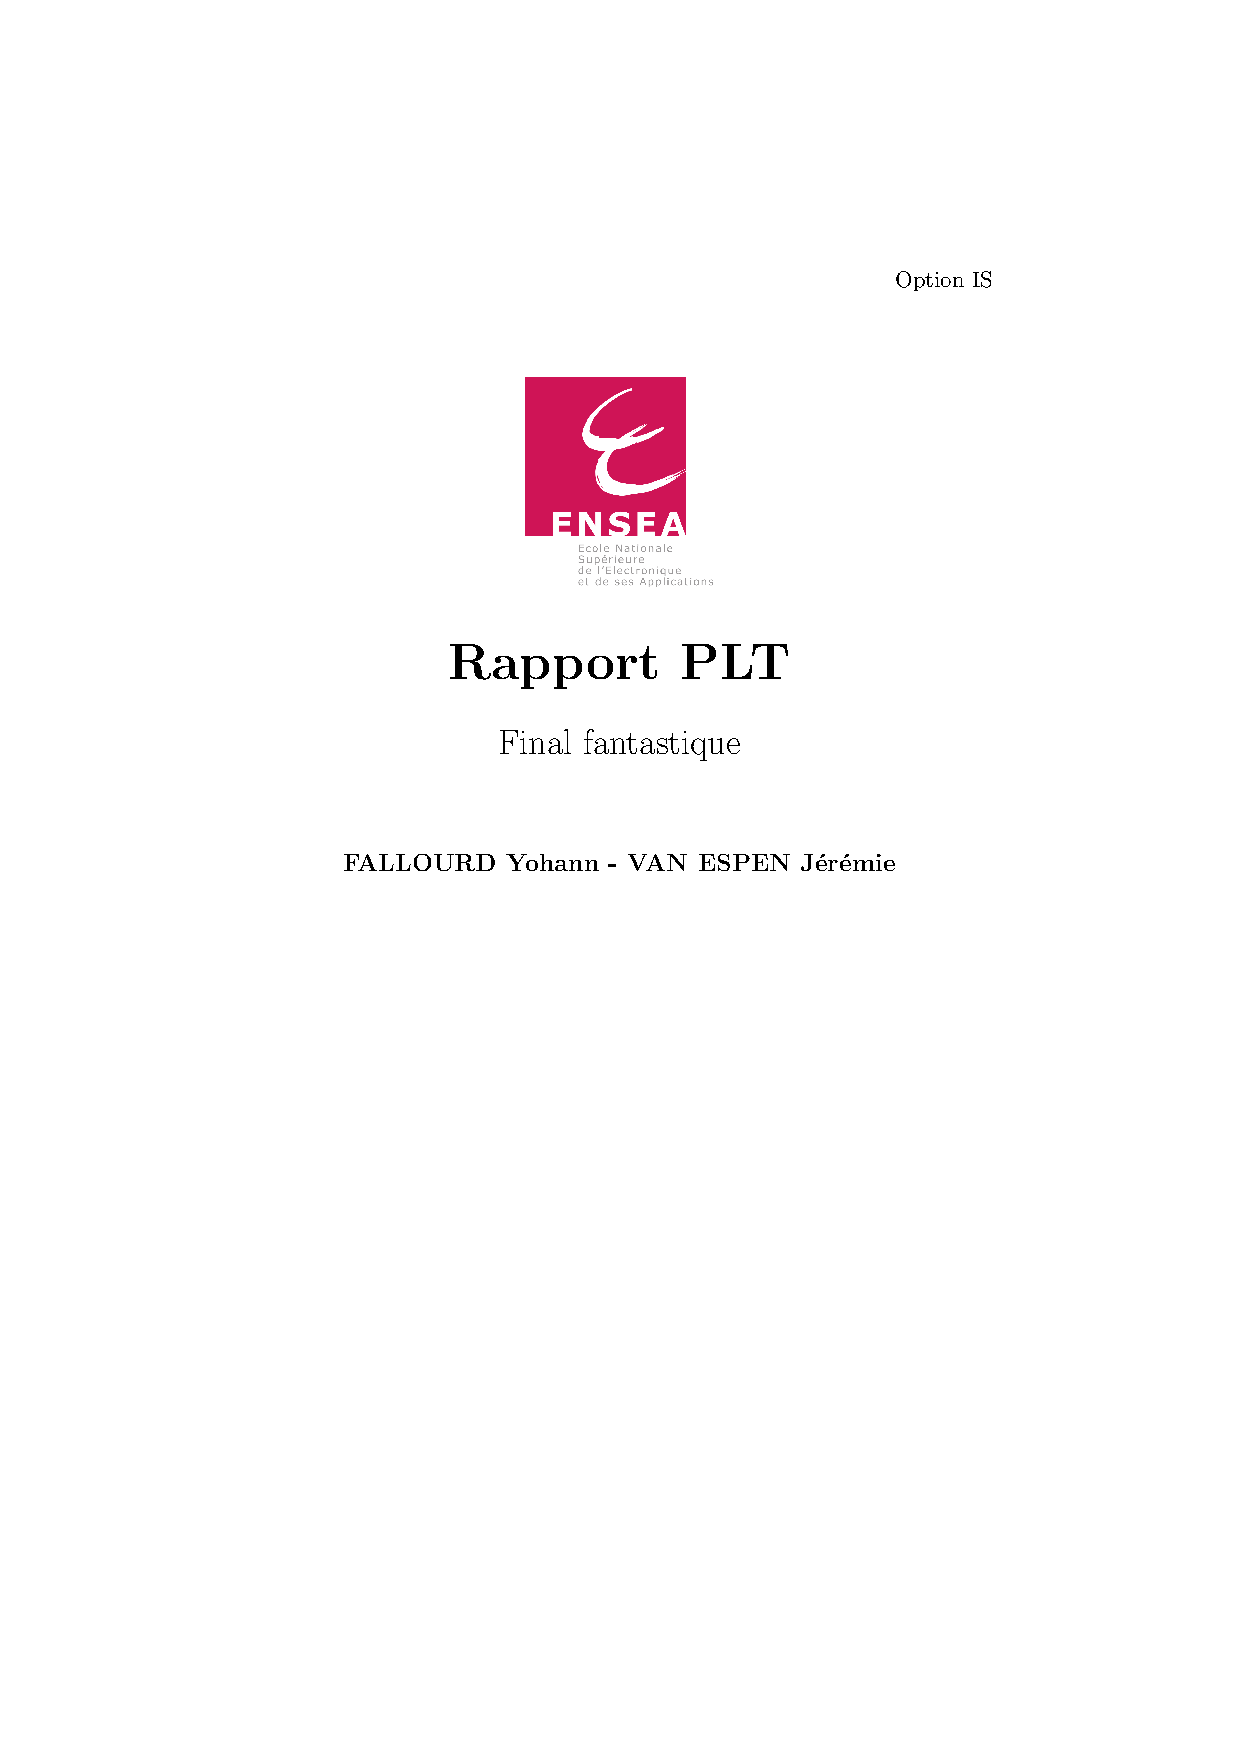
\includepdf{Titlepage}
\tableofcontents
\chapter{Objectif}
\section{Présentation générale}
Le jeu est bas\'{e} sur l'arch\'{e}type de Final Fantasy X, se distinguant par un système de combat au tour par tour ainsi que son embl\'{e}matique "sph\'{e}rier" correspondant à un arbre de talent apportant une libert\'{e} de personnalisation non n\'{e}gligeable. Voici un croquis du sphérier :

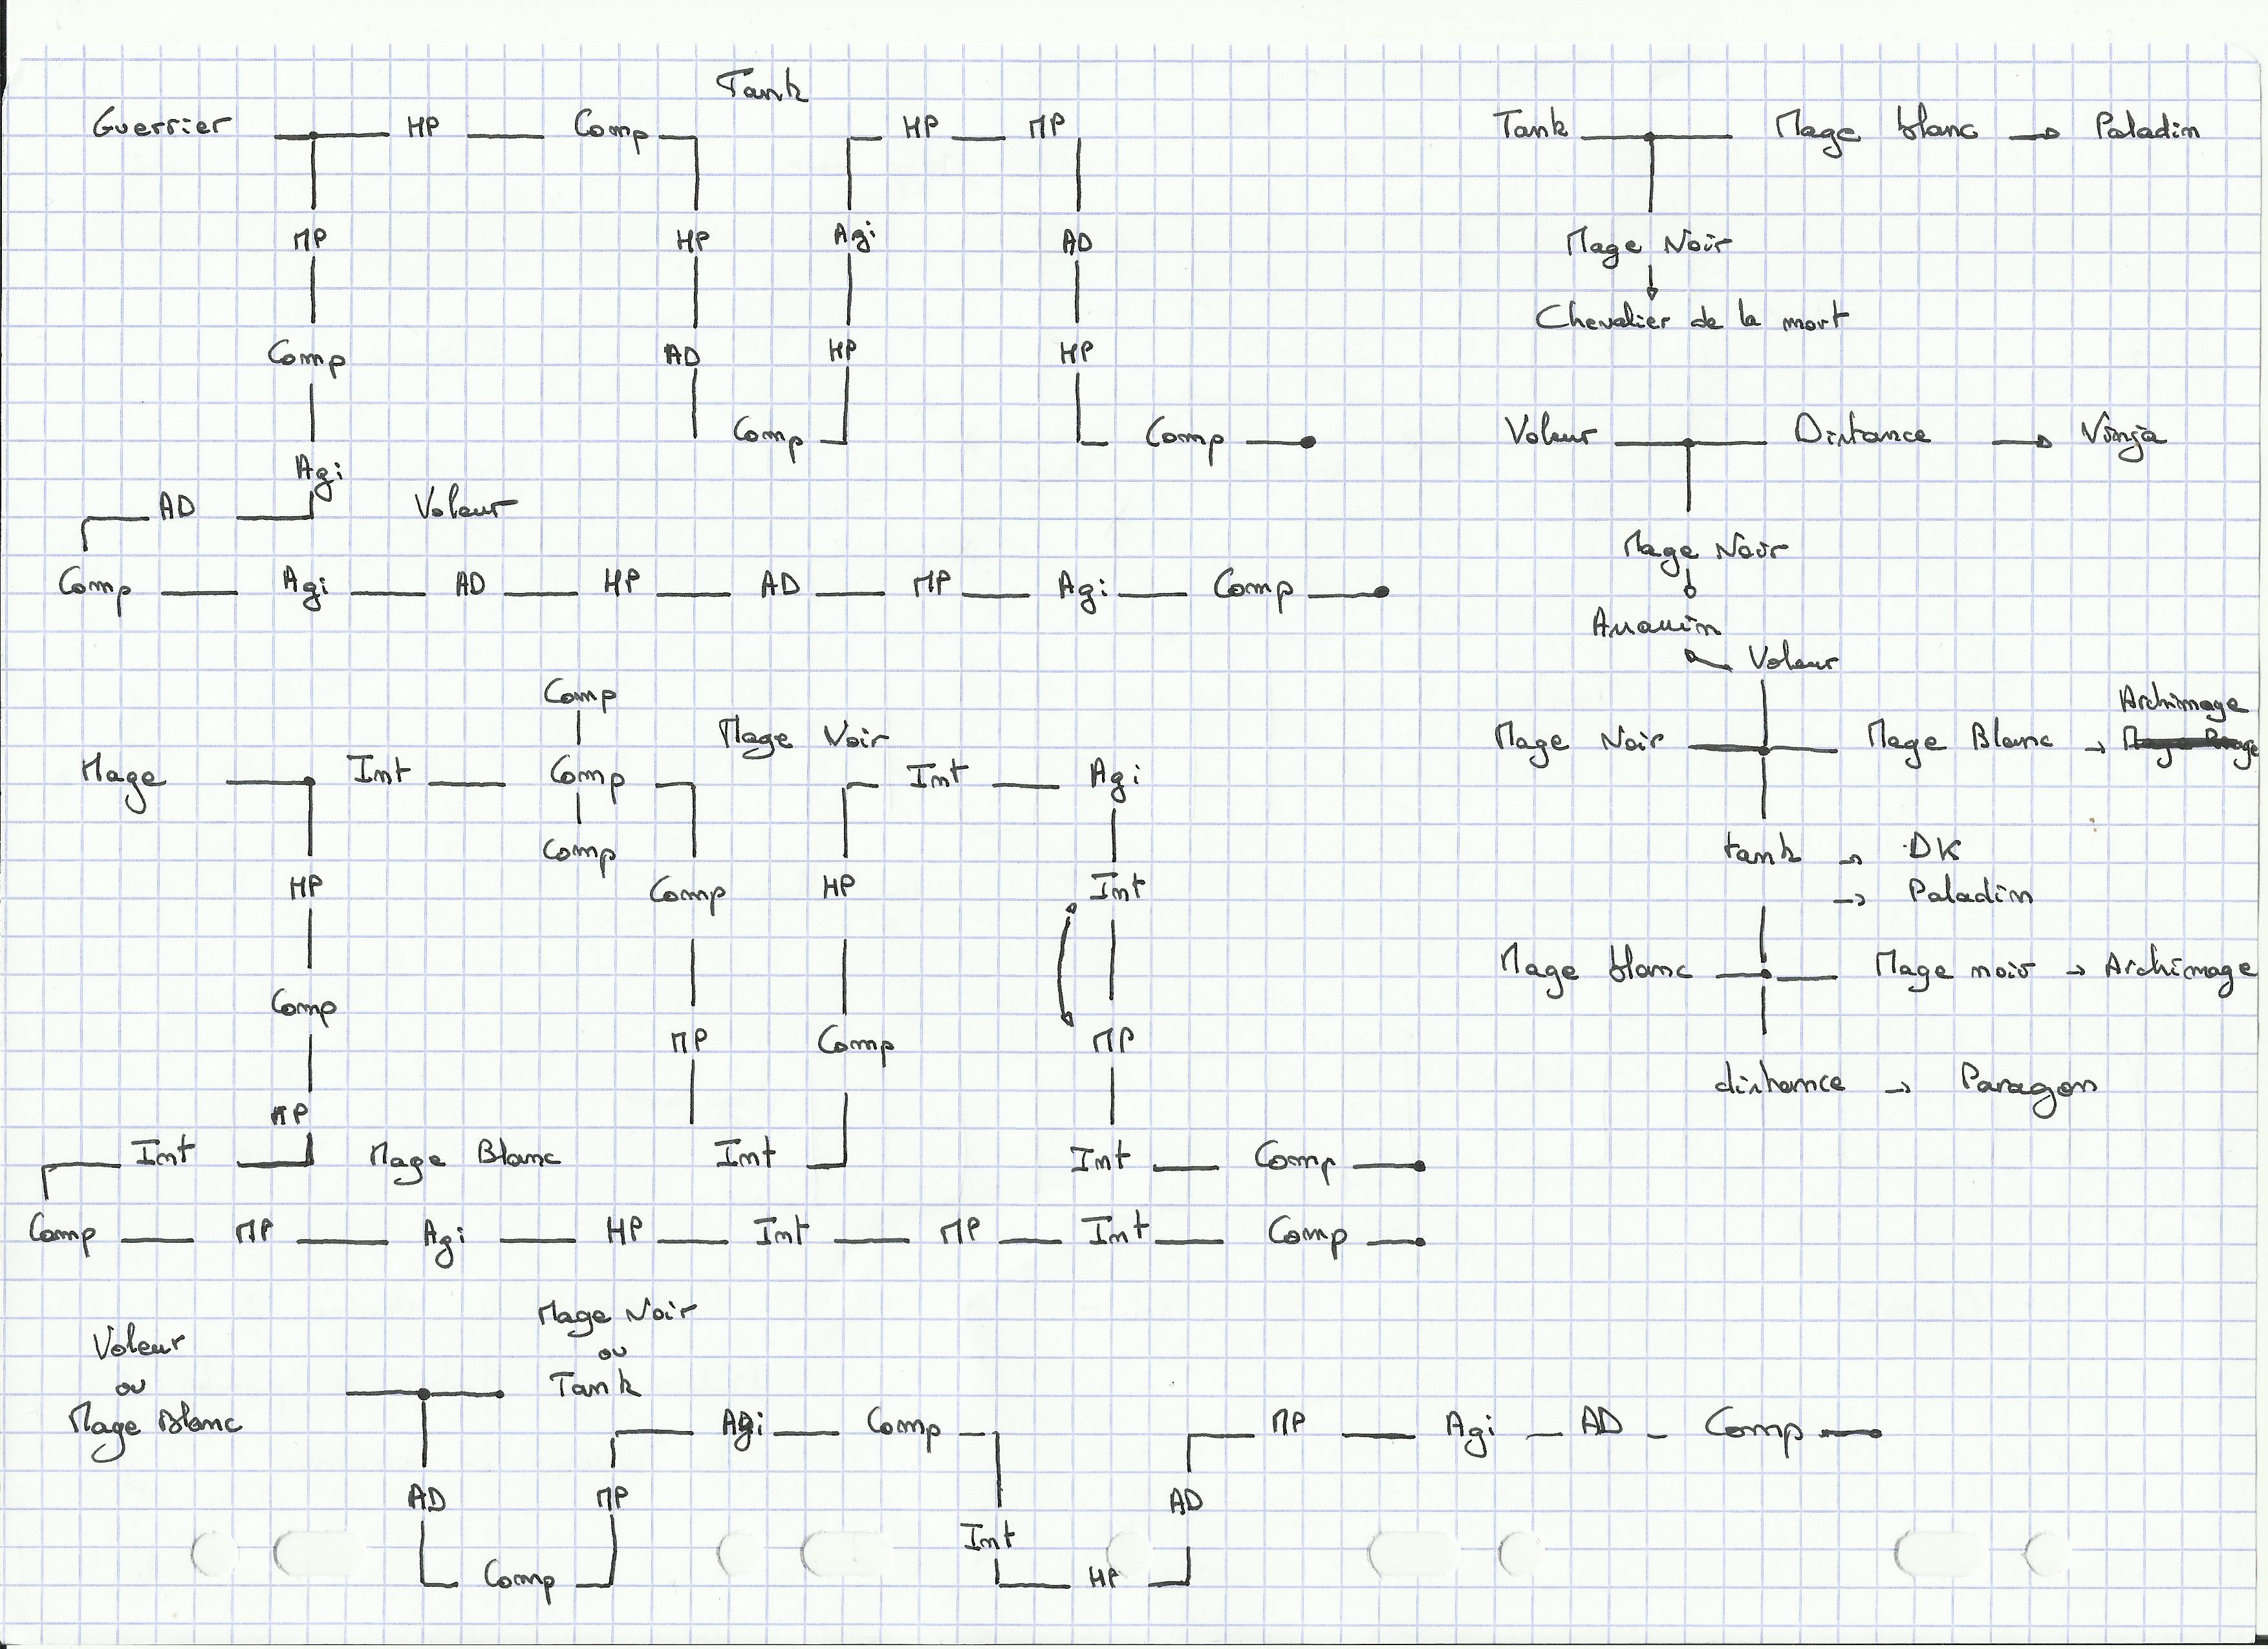
\includegraphics[width=0.80\textwidth]{Spherier.jpg}

A la diff\'{e}rence du v\'{e}ritable jeu, il n'y aura pas de d\'{e}placement libre en temps r\'{e}el; le gameplay se r\'{e}sume à un d\'{e}placement de points d'int\'{e}rêts en points d'int\'{e}rêts, poussé par une histoire typique de cet arch\'{e}type, où se déroulent diff\'{e}rents \'{e}vènements/combats.


\section{Règles du jeu}
Le coeur du jeu sont les deux personnages auquel le joueur (si il joue seul) a accès. Chacun commence avec une sp\'{e}cialisation particulière de mage et de guerrier choisissant directement de se diriger vers diff\'{e}rentes sp\'{e}cialisations. Via une carte du monde, le joueur avance de point en point et d\'{e}clenche diff\'{e}rentes rencontres. Les combats se d\'{e}roulent en tour par tour et si l'un des joueurs meurt, il revient à la vie avec 1 point de vie. La mort des deux joueurs entraine un retour au dernier point de sauvegarde automatique. Gagner un combat donne de l'exp\'{e}rience, qui donne des niveaux, qui permettent de progresser dans le sph\'{e}rier. 

Il existe \'{e}galement diff\'{e}rents objets permettant de rendre de la vie ou d'avoir d'autres effets. De plus, un système d'\'{e}quipement existe pour rendre le joueur plus fort au cours de l'aventure. En effet, un personnage possède des caract\'{e}ristiques (Force, Agilit\'{e}, Intelligence, Points de vie (HP) et Points de magie (MP)) qu'il peut am\'{e}liorer.

Le jeu se finit lorsque l'aventure est termin\'{e}e !
\section{Conception Logiciel}

Voici les packages de notre projet :

\textbf{Package state.} Package central qui gère l'\'{e}tat du jeu.

\textbf{Package engine.} Package qui modifie l'\'{e}tat de jeu en fonction de diff\'{e}rents inputs.

\textbf{Package ai.} Package qui gère le contrôle par l'ordinateur des monstres et, potentiellement, un personnage principal.

\textbf{Package server.} Package contenant la gestion de l'API du jeu, que ce soit par r\'{e}seau ou localement.

\textbf{Package instance.} Gère les différents contexte de jeu et leur rendu.

\textbf{Package client.} Package contenant les diff\'{e}rents traitements et commandes faites localement, sur la machine du joueur, afin de produire le comportement souhait\'{e} du jeu.

\textbf{Package entity.} Package contenant toutes les entit\'{e}s du jeu. Cela rassemble les Personnages Non Joueurs, les personnages principaux et les diff\'{e}rents ennemis.

\textbf{Package capacities.} Package contenant les diff\'{e}rents sorts et capacit\'{e}s utilis\'{e}es par les personnages principaux et les ennemis.

\begin{figure}
\caption{Diagramme des packages}
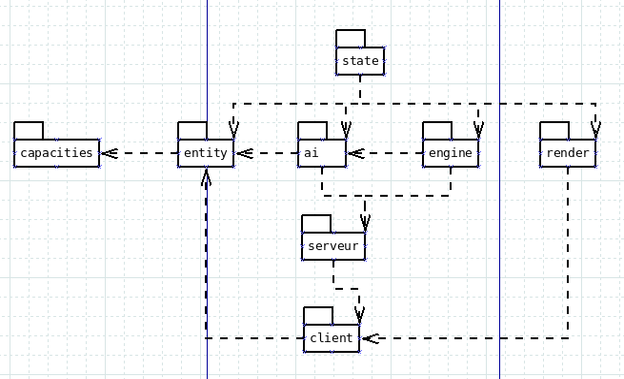
\includegraphics[width=0.80\textwidth]{lol.jpg}
\end{figure}

\chapter{Description et conception des \'{e}tats}
\section{Description des \'{e}tats}

Un \'{e}tat du jeu est form\'{e} par un ensemble d'\'{e}l\'{e}ments vivants et non vivants ainsi que la situation dont se trouve le joueur.

\subsection{Etat \'{e}l\'{e}ments vivants}

Les \'{e}l\'{e}ments vivants sont des entit\'{e}s ayant tous des caract\'{e}ristiques propres : santé max, santé actuelle, mana max, mana actuel, force, agilit\'{e} et intelligence.
On distingue deux types d'\'{e}l\'{e}ments vivants :

\textbf{Character.} Ce sont les h\'{e}ros du jeu. Ils pourront s'\'{e}quiper d'une arme et d'une protection ajoutant des bonus d'attaque et de d\'{e}fence. Ils \'{e}volueront grâce \`{a} un syst\`{e}me de gain d'exp\'{e}rience et de personalisation du joueur.  

\textbf{Monster.} Comme le nom l'indique, ce sont les monstres du jeu. Ils ne peuvent pas gagner d'exp\'{e}rience et leurs caract\'{e}ristiques sont g\'{e}n\'{e}r\'{e}es avec le niveau actuel des h\'{e}ros. Leurs comp\'{e}tences seront fix\'{e}es suivant le type du monstre (\'{e}l\'{e}mentaire, boss ect...). Ils ne portent pas d'\'{e}quipement. Seul les boss auront une capacit\'{e} sp\'{e}ciale (comme les h\'{e}ros) appel\'{e} "Overdrive".

\subsection{Etat \'{e}l\'{e}ments non vivants}

Les \'{e}l\'{e}ments non vivants sont au nombre de trois et ne portent aucune caract\'{e}ristiques communes. 

\textbf{Item.} Ce sont les objets utilisables par les h\'{e}ros. Ils peuvent changer leurs attributs (augmentation d'une caract\'{e}ristique ect...).

\textbf{Equipment.} Ce sont les armes et protections que peuvent poss\`{e}der les h\'{e}ros. Leurs effets seront pris en compte dans la m\'{e}thode Takedomage() présent dans la class Element.   

\textbf{Node.} Ce sont les points clefs du jeu. Les h\'{e}ros pourront se d\'{e}placer sur une carte de noeud en noeud. Chaque noeud comporte des \'{e}v\`{e}nements al\'{e}atoires et non al\'{e}atoires. Les \'{e}l\'{e}ments al\'{e}atoires sont des combats contre des monstres al\'{e}atoires tandis que les non al\'{e}atoires sont des \'{e}l\`{e}ments de l'histoire. Cela peut \^{e}tre un simple dialogue ou un combat contre un boss. Il est possible uniquement de ce d\'{e}placer au noeud suivant ou au noeud pr\'{e}c\'{e}dent. Si ce noeud a d\'{e}j\`{a} \'{e}t\'{e} visit\'{e}, l'\'{e}v\`{e}nement non al\'{e}atoire n'aura plus lieu.

\subsection{Situation du joueur}

Les situations possibles dans lequelles se trouve le joueur sont au nombre de quatre. Elles repr\'{e}sentent la ligne directive du jeu.

\textbf{D\'{e}placement sur un noeud.} Le joueur se d\'{e}place dans un nouvel endroit qui va g\'{e}n\'{e}rer des \'{e}v\`{e}nements. 

\textbf{Ev\`{e}nement al\'{e}atoire.} Cet \'{e}v\`{e}nement se traduit la plus part du temps par un combat contre des monstres al\'{e}atoires.

\textbf{Aubergiste.} En arrivant dans un nouveau lieu, le joueur a acc\`{e}s \`{a} un menu lui permettant d'acheter des objets utilisables en combat et de se pr\'{e}parer \`{a} l'\'{e}v\`{e}nement non al\'{e}atoire.

\textbf{Ev\'{e}nement non al\'{e}atoire.} Il d\'{e}pend de l'histoire du jeu.

\newpage

\section{Conception logiciel}

Dans cette section, nous expliciterons le diagrammes des classes pour les \'{e}tats pr\'{e}sent\'{e} en fin de chapitre. 

\textbf{Classes Element.} Cette classe et ses classes filles contiennent tout les \'{e}l\'{e}ments vivants du jeu. Elle est intras\`{e}quement li\'{e}e aux classes Capacities, Equipment et Spherier qui viennent compl\`{e}ter la classe Character. 

\textbf{Fabrique d'\'{e}l\'{e}ments.} Cette classe a pour but de rendre plus facile la construction d'\'{e}l\'{e}ments vivants, notamment des monstres provenant d'un \'{e}v\`{e}nement al\'{e}atoire (consid\'{e}r\'{e} comme non boss).

\textbf{Liste d'\'{e}l\'{e}ments.} Elle va contenir toute les informations sur l'ensemble des \'{e}l\'{e}ments pr\'{e}sent dans le jeu. 

\textbf{Classes Node.} Cette classe permet de faire le lien entre l'apparition d'\'{e}v\`{e}nements et les \'{e}l\'{e}ments. C'est une liste chain\'{e}e dont le d\'{e}placement est bidirectionnel.

\textbf{Fabrique de noeuds.} Nous reprenons le m\^{e}me sch\'{e}ma que la classe Element et les classes li\'{e}es \`{a} celle-ci. Ainsi la fabrique de noeuds permettra une mise en place plus facile des points clefs du jeu.

\textbf{Liste de noeuds.} Elle va contenir toute les informations sur l'ensemble des noeuds pr\'{e}sent dans le jeu. 

\textbf{Classe State.} Cette contiendra toutes les informations li\'{e}es aux noeuds et aux \'{e}l\'{e}ments vivants / non vivants.

\begin{sidewaysfigure}[ht]
\caption{Diagramme des classes du package State}
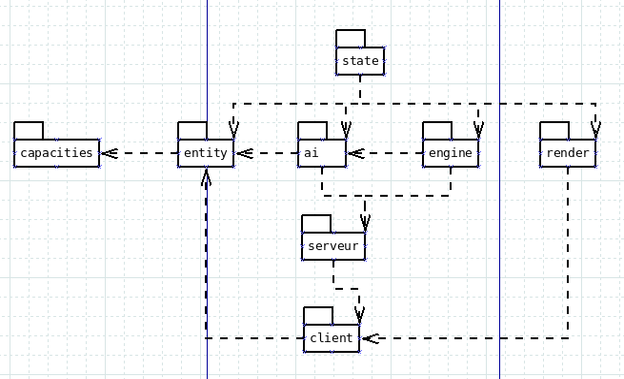
\includegraphics[width=1.25\textwidth]{lol.jpg}
\end{sidewaysfigure}


\chapter{Rendu : Stratégie et Conception}
\section{Stratégie de rendu d'un état}
Notre jeu étant à temps discret, le rendu d'un état sera assez simple. Le tout étant de distinguer entre un changement d'état qui n'entraîne pas un lourd besoin de rendu (ie. pendant un combat) et un changement d'état demandant un changement de sprites (ie. changer de ville).

Pour se faire, nous introduisons le concept d'instance, offrant une classe par contexte (ie. Combat, Carte du monde, Menu d'intro...) gérant la logique d'initialisation ainsi que le rendu de ce contexte utilisant les méthodes de SFML.
\section{Conception logiciel}

\section{Conception logiciel : extension pour les animations} 


\end{document}
